\chapter{Results}

The analysis will be split into two parts. The first part focuses on the probabilities and frequencies of coincident events, while the second part 
consists of a detailed analysis of the data aquired by the FRT. 

\section{Probabilities of coincident events}\label{sec:muon_coincidence}

\section{Analysis of the Fixed Rate Trigger}

As mentioned in section~\ref{sec:daq}, the FRT has a comparatively large readout window of \SI{10}{ms}. The result of this is that one \textit{event} contains 
a substantial amount of DOM hits. Since the average muon rate in IceCube is around \num{2200}\unit{Hz}, there is a significant likelihood, that any \textit{event}
contains physically significant signals. Other than muon events, there might be neutrino events as well as other possible atmospheric or astrophysical signals 
being measured in a given readout window of the FRT. However, a major fraction of the signals detected by the FRT is expected to be noise. 
(wie gibt man den Datensatz an, gibt es da einen standart?). The subsequent analysis is an attempt to extract knowledge about the composition of the signals 
measured by FRT and to possibly use them to better understand coincident events in IceCube.\\

The first step breaking down the FRT's data is to inspect the kind of signals detected during a single \textit{event}. In accordance with the description of 
\textit{subevents} in \ref{sec:daq}, a python script is used to filter out the corresponding signals (detaillierter~?). Depicted in 
figure~\ref{fig:frt_mu_sub_comp_1} is a comparison of the unfiltered signals of an event and the filtered signals. Most notably, the two distributions show a 
general similarity between them. As expected, there are substantially more unfiltered signals than filtered signals, showing that there are infact signals 
being filtered. The filtered \textit{subevents} contain \SI{47}{\percent} of the total signals. The expectation would be to see a clear shift towards higher 
charge values in distribution of filtered signals, based on the idea that signals which stem from astrophysical or atmospheric sources would carry higher energy 
than noise signals. The observation does not quite match this expectation.
\begin{figure}[H]
    \centering
    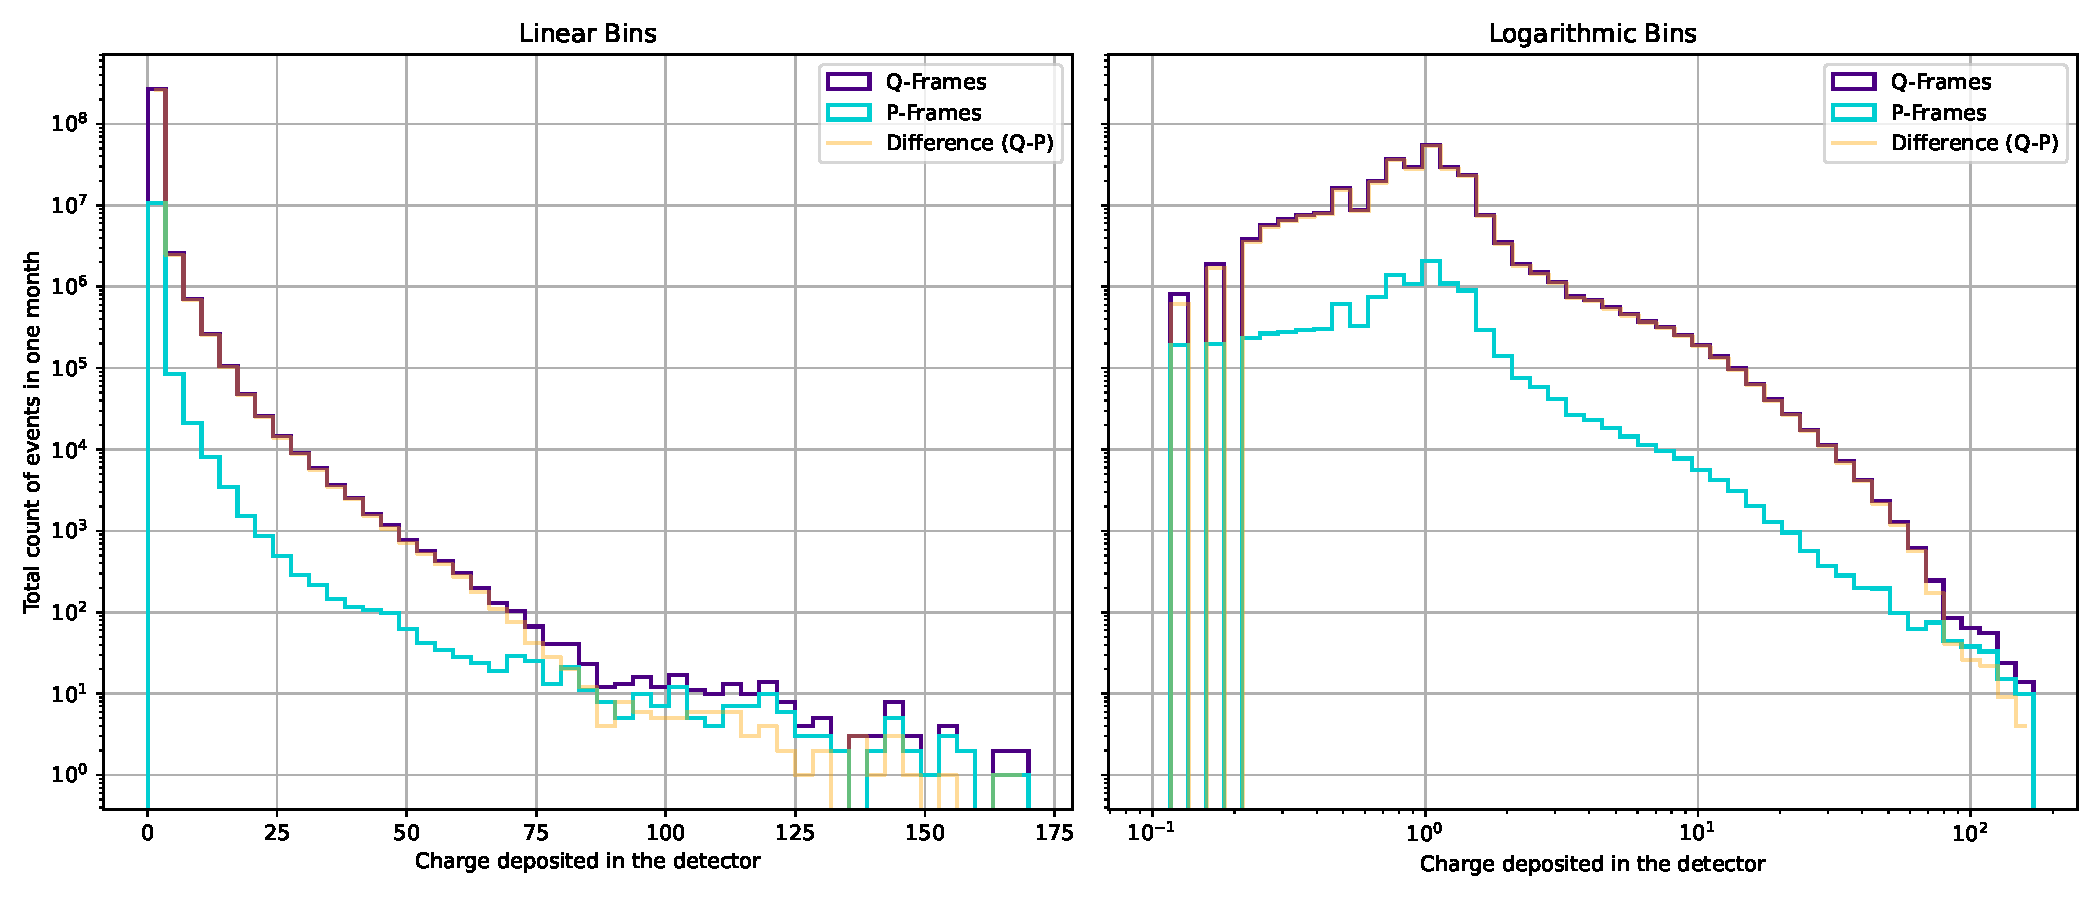
\includegraphics[width=\textwidth]{Plots/q_p_comp.pdf}
    \caption{A comparison between the counts of all Signals and physics signals.}
    \label{fig:frt_mu_sub_comp_1}
\end{figure}

